\subsection{Partes} \label{subsec:partes}
%Aquí pondrán la información de las piezas del robot. Pueden eliminar las siguientes subsecciones y simplemente explicar los motores usados y el material de los eslabones porque ya no hay tiempo.
\subsubsection{Motores} \label{subsubsec:motores}
%Explicarán cuál es el motor que usaron, harán referencia a la hoja de datos, así como las transmisiones (por ejemplo, las de las pinzas) o reductores de velocidad a los que están acoplados. Deben de poner también información como: masa, fuerza o torque máximo, razón de reducción (por ejemplo, 10/1) y la velocidad máxima.
\subsubsection{Selección del Motor y Sistema de Transmisión}

Para el diseño del robot con una altura aproximada de 1.5 metros y un peso total de 272 kg, se optó por motores de corriente continua de alto torque acoplados a \textbf{reductores planetarios}, los cuales garantizan la fuerza y el control necesarios para manipular el cuerpo del robot, sus articulaciones y herramientas (como pinzas).

\paragraph{Motores Principales.}

\begin{itemize}
	\item \textbf{Modelo:} DC Motor MY1020 (Brush Motor)
	\item \textbf{Hoja de datos:} Disponible en \url{https://www.cnnbmotor.com}
	\item \textbf{Tensión nominal:} 24 V
	\item \textbf{Potencia nominal:} 500 W
	\item \textbf{Torque máximo:} 2.2 Nm (directo del eje del motor)
	\item \textbf{Velocidad sin carga:} 3000 rpm
	\item \textbf{Corriente nominal:} 26 A
	\item \textbf{Masa del motor:} 4.8 kg
\end{itemize}

Este motor es utilizado para los movimientos de desplazamiento del robot y para otras articulaciones que requieren potencia constante.

\paragraph{Reductores de Velocidad.}

Para garantizar un movimiento controlado y con mayor torque, el motor MY1020 está acoplado a un \textbf{reductor planetario} de relación 20:1:

\begin{itemize}
	\item \textbf{Tipo:} Reductor planetario
	\item \textbf{Relación de reducción:} 20:1
	\item \textbf{Torque de salida (post reductor):} 44 Nm
	\item \textbf{Velocidad de salida:} 150 rpm aprox.
	\item \textbf{Masa del reductor:} 3.2 kg
\end{itemize}

\paragraph{Motores para Pinzas o Ejes Menores.}

Para el sistema de pinzas del robot o movimientos más pequeños, se utilizó el \textbf{servomotor MG996R}:

\begin{itemize}
	\item \textbf{Modelo:} MG996R Servo
	\item \textbf{Voltaje de operación:} 4.8 – 7.2 V
	\item \textbf{Torque máximo:} 11 kg·cm ($\approx$ 1.08 Nm a 6 V)
	\item \textbf{Velocidad:} 0.14 s/60° a 6 V
	\item \textbf{Tipo de control:} PWM
	\item \textbf{Ángulo de operación:} 0–180°
	\item \textbf{Peso del servomotor:} 55 g
\end{itemize}

Estos servos permiten el control de precisión en mecanismos como pinzas, pequeños actuadores o movimientos secundarios.

\paragraph{Justificación de Selección.}

El motor \textbf{MY1020 con reductor} proporciona suficiente torque para mover estructuras pesadas como los brazos o el cuerpo del robot, permitiendo además un control fino gracias al uso de controladores PWM o puentes H.

Los \textbf{servos MG996R}, aunque más pequeños, son confiables, económicos y eficaces para tareas que requieren exactitud y bajo torque.

La combinación permite un diseño \textbf{modular}, balanceado entre \textbf{potencia}, \textbf{control} y \textbf{eficiencia energética}.

\subsubsection{Eslabones} \label{subsubsec:eslabones}
	\begin{figure}[H]
	\centering
	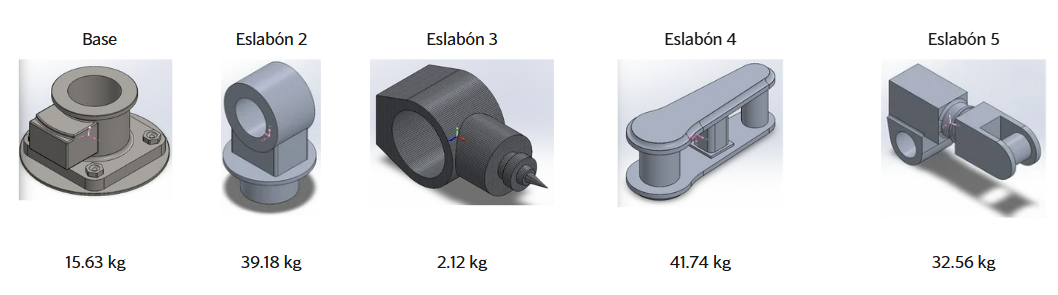
\includegraphics[width=0.7\textwidth]{img/Eslabones.png}
	\caption{Eslabones del robot}
	\label{fig:Eslabones}
\end{figure}

\subsubsection{Propiedades Físicas de los Eslabones y la Base}
\paragraph{Base}
\begin{itemize}
	\item \textbf{Masa:} 156.3841 kg
	\item \textbf{Material:} Acero al carbono fundido
	\item \textbf{Longitud e inercia:} No especificadas
\end{itemize}
\paragraph{Eslabón 2}
\begin{itemize}
	\item \textbf{Longitud:} 1.30 m
	\item \textbf{Masa:} 39.1896 kg
	\item \textbf{Inercia:} 2.6673 kg$\cdot$m$^2$
	\item \textbf{Material:} Aleación de aluminio 6061
\end{itemize}

\paragraph{Eslabón 3}
\begin{itemize}
	\item \textbf{Longitud:} 1.30 m
	\item \textbf{Masa:} 41.7432 kg
	\item \textbf{Inercia:} 3.0513 kg$\cdot$m$^2$
	\item \textbf{Material:} Aleación de aluminio 6061
\end{itemize}

\paragraph{Eslabón 4}
\begin{itemize}
	\item \textbf{Longitud:} 1.00 m
	\item \textbf{Masa:} 32.5622 kg
	\item \textbf{Inercia:} 1.6734 kg$\cdot$m$^2$
	\item \textbf{Material:} Aleación de aluminio 6061
\end{itemize}

\paragraph{Eslabón 5}
\begin{itemize}
	\item \textbf{Longitud:} 0.40 m
	\item \textbf{Masa:} 2.1294 kg
	\item \textbf{Inercia:} 0.0281 kg$\cdot$m$^2$
	\item \textbf{Material:} Fibra de carbono
\end{itemize}


